\documentclass{article}
\usepackage[utf8]{inputenc}
\usepackage[spanish,mexico]{babel}
\usepackage[margin=2.5cm]{geometry}
\usepackage{graphicx}
\usepackage[export]{adjustbox}
\usepackage{caption}
\usepackage{subcaption}
\usepackage{fancyhdr}
\usepackage{enumitem}
\usepackage{amsmath}
\usepackage{amssymb}
\usepackage{amsfonts}
\usepackage{hyperref}
\pagestyle{fancy}
\fancyhf{}

\title{Template Facultad de Ciencias, UNAM}
\author{Isidro Armando de Ojalvo Abelló García}
\date{\today}

\begin{document}

\thispagestyle{empty}

	\begin{figure}[ht]
	   \minipage{0.76\textwidth}
			
\includegraphics[width=4cm]{Logo_UNAM.png}
			\label{EscudoUNAM}
	   \endminipage
	   \minipage{0.32\textwidth}
			
\includegraphics[height=4.3cm ,width=4.3cm]{Logo_FC.png}
			\label{EscudoFC}
		\endminipage
	\end{figure}

	\begin{center}
	\vspace{0.8cm}
	\LARGE
	UNIVERSIDAD NACIONAL AUTÓNOMA DE MÉXICO

	\vspace{0.8cm}
	\LARGE
	FACULTAD DE CIENCIAS

	\vspace{1.7cm}
	\Large
	\textbf{REPORTE\\ Primer Proyecto: OjalvoChat}

	\vspace{1.3cm}
	\normalsize
	PRESENTA \\
	\vspace{.3cm}
	\large
	\textbf{Isidro Armando Abelló García \\ 426009038}

	\vspace{1.3cm}
	\normalsize
	PROFESOR \\
	\vspace{.3cm}
	\large
	\textbf{Dr. Canek Peláez Valdés}

	\vspace{1.3cm}
	\normalsize
	ASIGNATURA \\
	\vspace{.3cm}
	\large
	\textbf{Modelado y Programación}

	\vspace{1.3cm}
	\today
	\end{center}

	\newpage

    \section{Introducción}

    Este primer proyecto de la asignatura de Modelado y Programación consistió en la creación de un servidor y un cliente de chat basados en un protocolo previamente establecido. El sistema permite gestionar conexiones simultáneas con múltiples clientes, así como la administración de usuarios.

    En las secciones siguientes se presenta el análisis del problema, el modelo empleado para representar sus componentes, una descripción del proceso de desarrollo y, finalmente, las conclusiones obtenidas.

    \section{Análisis del problema}

    El proyecto consistió en desarrollar un sistema de chat que cumpliera con distintos requerimientos, entre los cuales destacaban principalmente el protocolo proporcionado por el profesor y el uso obligatorio de hilos de ejecución en el servidor, además de que las conexiones debían establecerse a nivel de sockets. De los puntos extra propuestos por el profesor, decidí intentar, en primera instancia, programar el servidor en C, emplear lenguajes distintos para el servidor y el cliente, realizar pruebas unitarias y llevar a cabo el desarrollo orientado a pruebas (TDD, por sus siglas en inglés). Con esto quedaron establecidos, a grandes rasgos, los requerimientos del proyecto, por lo que procedí a trabajar en él.\\

    A partir de este planteamiento identifiqué los siguientes subproblemas, los cuales aborde en el orden que se presenta a continuación:

    \begin{enumerate}
        \item Aprender a utilizar múltiples hilos de ejecución.
        \item Aprender a establecer conexiones a nivel de sockets.
        \item Aprender los fundamentos y las buenas prácticas de programación del lenguaje C.
        \item Encontrar un sistema de construcción adecuado para C.
        \item Aprender a realizar pruebas unitarias en C.
        \item Establecer una estructura que administre al servidor.
        \item Recibir correctamente los mensajes entre servidor y cliente a través del protocolo TCP.
        \item Investigar alguna biblioteca que permitiera manejar JSON en C.
        \item Mantener la conexión con los clientes y desconectarlos en caso de comportamientos fuera del protocolo.
        \item Modelar las estructuras necesarias para manejar mensajes, usuarios, listas de usuarios, salas y listas de salas.
        \item Comunicar, en el núcleo del modelo, todas estas estructuras de manera que se cumpliera el protocolo, garantizando la seguridad en un entorno de múltiples hilos de ejecución.
        \item Desarrollar un cliente funcional y seguro para el servidor.
        \item Manejar las estructuras de mensajes en el cliente.
        \item Dotar al cliente de la capacidad de leer correctamente los mensajes del servidor y de escribir mensajes hacia este.
    \end{enumerate}

    Para el momento en que se orientó el proyecto no conocía nada sobre múltiples hilos de ejecución ni sobre la conexión mediante sockets, así que lo primero que hice fue investigar el funcionamiento general de ambos temas. Una vez comprendidos los conceptos básicos de estas tecnologías, me dediqué a aprender los fundamentos de C, pues nunca había trabajado con este lenguaje. Al ser C un lenguaje de programación estructurada —paradigma en el que nunca había desarrollado un proyecto de gran tamaño— intenté, en un inicio, encontrar la manera de emular la orientación a objetos dentro de él. A pesar de que existen distintas herramientas que en apariencia logran este propósito, me parecieron complicadas, al menos con los conocimientos de C que tenía en ese momento, por lo que decidí emplear el paradigma estructurado, propio del lenguaje, para el desarrollo del proyecto. Con estos planteamientos y decisiones, quedé listo para diseñar el proyecto.

    \section{Diseño}

    Para diseñar el proyecto se dan respuestas más técnicas a la enumeración de problemas analizada anteriormente.

    \begin{itemize}
        \item La manera más adecuada de emplear múltiples hilos de ejecución en el programa consiste en asignar un hilo para ejecutar el ciclo de vida de un mensaje cada vez que un cliente lo envía.
        \item Dado que cada cliente cuenta con un descriptor de archivo (\textit{file descriptor}) específico y único para un puerto determinado, a través del cual llegan y se envían los mensajes, es necesario asociar a los clientes con su respectiva conexión.
        \item El lenguaje $C$ puede trabajarse de manera relativamente eficiente siempre que se administren correctamente la memoria y los errores. Existen diversas técnicas que se aprenden principalmente a través de la práctica y que resultan difíciles de anticipar de antemano.
        \item El sistema de construcción elegido fue \textit{Meson}, ya que cumple con los requerimientos de compilación, importación de bibliotecas y ejecución de pruebas, que eran los aspectos básicos que necesitaba.
        \item La biblioteca \textit{Criterion} permite manejar adecuadamente las pruebas unitarias en \textit{C}.
        \item La biblioteca \textit{cJSON} permite manejar adecuadamente los archivos \textit{JSON} en \textit{C}.
        \item Aprendí a crear estructuras en $C$ mediante el uso de \textit{headers} y la declaración de \textit{typedef}, lo cual permitió administrar las estructuras necesarias; en particular, el servidor cuenta con su puerto, socket, lista de usuarios y lista de salas, cuyos métodos principales sirven para aceptar, desconectar y enviar mensajes a los clientes. En esta parte se aplicó de manera extensa lo aprendido sobre sockets y conexiones.
        \item Para manejar la conexión con los clientes se implementó, ya en un entorno de múltiples hilos de ejecución, la función \textit{client\_handler}, encargada de revisar continuamente los mensajes provenientes de los clientes. Esta función utiliza la estructura auxiliar \textit{message\_buffer}, que obtiene el texto crudo enviado por el cliente y lo almacena, para posteriormente extraer, a partir de los separadores de línea, cada mensaje de manera individual. Una vez obtenido un mensaje, se intenta convertir a JSON mediante la biblioteca \textit{cJSON}. Si el mensaje cumple con el protocolo, se envía a procesar.
        \item Para la estructura de los mensajes seguí el consejo del profesor de incluir todas las propiedades posibles. Los tipos de mensajes se modelan mediante un \textit{enum}. Los métodos principales permiten convertir de cadena cruda a mensaje y de mensaje a cadena cruda (JSON).
        \item Para modelar la estructura de usuario se consideraron las propiedades de nombre, socket y estado.
        \item La estructura de la lista de usuarios es un doble \textit{Adapter} sobre las tablas de dispersión de \textit{glib}. Es doble porque permite buscar usuarios en $O(1)$ tanto por su nombre como por su socket. Implementa el patrón de diseño \textit{Iterator}, así como un método \textit{foreach} que aplica los patrones \textit{Visitor} y \textit{Adapter}. Además, es segura en un entorno de múltiples hilos, pues cada vez que se realiza una consulta o modificación, la estructura se bloquea mediante un \textit{mutex}, el cual se libera al finalizar el proceso.
        \item Para manejar las salas se creó una estructura que contiene el nombre de la sala y dos listas de usuarios: una de invitados y otra de miembros.
        \item La lista de salas es otro \textit{Adapter} sobre la tabla de dispersión de \textit{glib}, modelada de manera similar a la lista de usuarios en cuanto al manejo de múltiples hilos; cuenta con un método \textit{foreach} y con un \textit{Visitor} para una sala específica.
        \item La estructura encargada de manejar los mensajes es el \textit{message\_handler}, cuya función principal es reconocer el tipo de mensaje y, a partir de este, ejecutar el proceso correspondiente. Esta estructura constituye el núcleo del modelo, pues es donde realmente se implementa el protocolo.
        \item El cliente está escrito en $C\#$, un lenguaje orientado a objetos, en el cual se empleó el patrón de diseño Modelo--Vista--Controlador (MVC). El modelo del cliente consiste en la clase abstracta \textit{Mensaje}, que representa los mensajes provenientes del servidor, mientras que las implementaciones específicas corresponden a las clases que representan cada tipo de mensaje. La vista es una clase encargada de mostrar en consola todos los menús y mensajes del servidor. El controlador se encarga, simultáneamente, de recibir los mensajes que llegan del servidor y de atender la consola para que el usuario pueda escribir el mensaje que desea enviar al servidor.
    \end{itemize}

    El diseño final del programa está condicionado, en gran medida, por el descubrimiento de nuevas técnicas y por los problemas inesperados que surgieron durante el proceso de desarrollo del proyecto.\\

\subsection{Diagramas de responsabilidades de las estructuras del servidor}

    \renewcommand{\arraystretch}{1.3}

    \newcommand{\crc}[2]
    {%
        \begin{tabular}{|l|l|}
            \hline
            \multicolumn{2}{|c|}{#1} \\
            \hline
            #2
            \hline
        \end{tabular}%
    }

    \begin{center}
        \mbox{%
        \crc{Message}
        {%
            mensaje del protocolo & Message\_Buffer \\
            parse JSON a Message & User, Room \\
            parse Message a JSON & Server \\
        }%

        \hspace{0.5cm}%

        \crc{User}
        {%
            datos del & Users\_Table \\
            usuario: nombre & Room \\
            socket, estado & Server \\
        }%

        \hspace{0.5cm}%
    }
\end{center}
\begin{center}
        \mbox{%
        \crc{Users\_Table}
        {%
            colección de usuarios & User \\
            búsqueda por nombre, socket & Server \\
            agregar, eliminar, recorrer colección & Room\_Table \\
            acceso seguro entorno multi-hilo &  \\
        }%

        \hspace{0.5cm}%

        \crc{Room}
        {%
            nombre, invitados & User \\
            miembros, agregar, & Room\_Table \\
            eliminar, acceder,  & Message \\
        }%
    }
\end{center}
\begin{center}
        \mbox{%
        \crc{Server}
        {%
            aceptar nuevas conexiones & Users\_Table \\
            administrar la recepción y desconexión & Room\_Table \\
            enviar mensajes & Message \\
        }%

        \hspace{0.5cm}%

        \crc{Room\_Table}
        {%
            colección de salas & Room \\
            buscar y actuar en sala & Server \\
            Agregar, eliminar y recorrer & Users\_Table \\
            acceso seguro en multi-hilo & \\
        }%
    }
\end{center}

\newpage

\subsection{Diagramas de actividades del servidor}

    \begin{figure}[h]
        \centering
        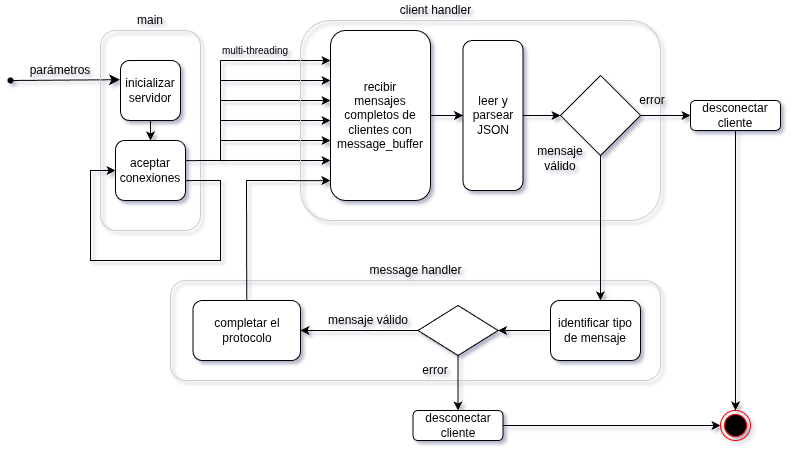
\includegraphics[scale=.6]{actividades.png}
        \caption{actividades del servidor.}
        \label{fig:diagrama}
    \end{figure}
    \vspace{2cm}
    \begin{figure}[h]
        \centering
        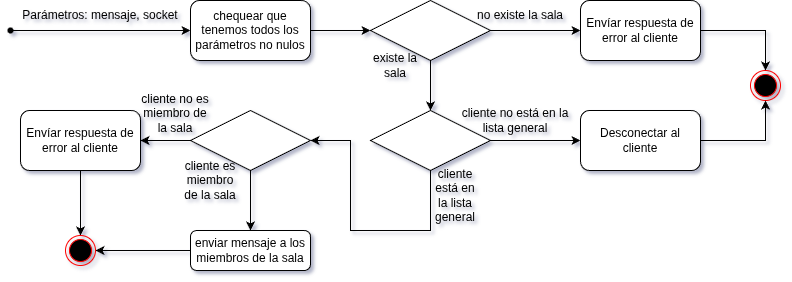
\includegraphics[scale=.5]{protocolo_room_text.png}
        \caption{actividades para el protocolo ROOM\_TEXT.}
        \label{fig:diagrama}
    \end{figure}

\newpage

\subsection{Diagrama UML del cliente}

    \begin{figure}[h]
        \centering
        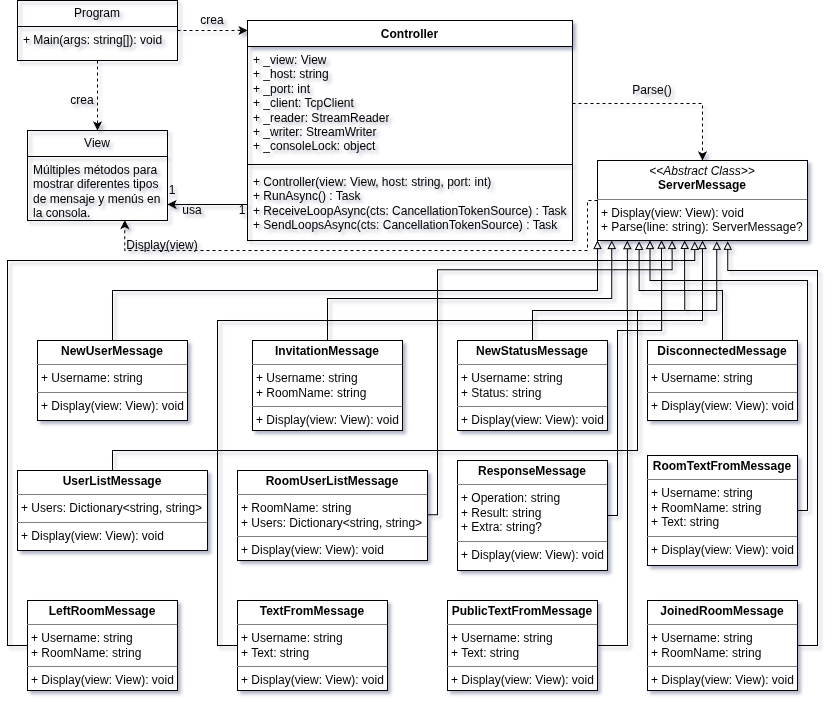
\includegraphics[scale=.5]{uml.png}
        \caption{UML.}
        \label{fig:diagrama}
    \end{figure}

    \section{Breve historia del desarrollo del proyecto}

    Una vez dominados los conceptos básicos de $C$, \textit{Meson} y \textit{Criterion}, tomé como referencia el código de un servidor de juguete y comencé a modelarlo de acuerdo con lo que buscaba; asimismo, escribí un cliente que únicamente se conectaba y se cerraba después de ello. Posteriormente, agregué al servidor banderas que permitieran ejecutarlo con distintos parámetros.

    Después separé al servidor en su propia estructura, en la cual implementé sus métodos básicos, pues hasta ese momento se encontraba incrustado en la función \textit{main}, la cual quedó únicamente como punto de entrada y controlador del servidor. En esta etapa también agregué mi primera prueba unitaria.

    En un inicio no pretendía incluir la estructura \textit{message\_buffer}; sin embargo, en una conversación con mi compañero Giovanni, este me comentó que, en ocasiones, los mensajes enviados por el cliente no llegaban completos. Por ello, decidí implementar dicha estructura antes de continuar, con el fin de resolver este problema y, al mismo tiempo, contar con un punto intermedio entre los JSON crudos recibidos de los clientes y la estructura de mensaje que pretendía implementar. Programar esta estructura resultó complicado debido al manejo intensivo de memoria que requiere, y tuve que aprender a realizar muchas tareas que en un lenguaje de más alto nivel hubiera pasado por alto; las pruebas unitarias me ayudaron considerablemente a verificar que lo que estaba escribiendo funcionara correctamente.

    A continuación, agregué la capacidad de múltiples hilos de ejecución al servidor y la probé con el cliente de juguete. Además, hice que el servidor se apagara de forma controlada mediante la señal del sistema Ctrl+C. Por no revisar adecuadamente una biblioteca que estaba utilizando, se presentó un error donde no se reconocían como válidos varios caracteres UTF-8; dicho error fue detectado y corregido oportunamente.

    Implementé la capacidad del servidor para recibir mensajes del cliente de juguete y responder con un eco del mismo mensaje. Posteriormente, implementé las estructuras de mensajes, usuarios y lista de usuarios conforme a lo establecido en el diseño, y a todas ellas les escribí las correspondientes pruebas unitarias. Con esto, ya era posible convertir cadenas crudas de JSON a mi estructura de mensajes, así como enviar dicha estructura en formato JSON.

    Después escribí el \textit{message\_handler}, comenzando con el proceso correspondiente al primer mensaje del protocolo: IDENTIFY. Al probar esta funcionalidad, me encontré con un error característico de $C$: al asignar ciertos literales, el programa fallaba debido a un \textit{double-free} en otra parte del código; el problema se resolvió empleando la función \texttt{strdup()} en la asignación correspondiente. En esta etapa también agregué una prueba de concurrencia para las listas de usuarios.

    Posteriormente incorporé la búsqueda doble en $O(1)$ en la lista de usuarios; gracias al encapsulamiento previamente logrado, escalar esta estructura resultó relativamente sencillo, pues bastó con agregar una segunda tabla de hash, vinculada con la primera, cuya llave fuera el descriptor de archivo del usuario.

    A continuación, implementé casi por completo el protocolo del mensaje de tipo DISCONNECT, seguido del de tipo STATUS. En este punto corregí también un caso de identificación falsa, en el cual un mismo cliente podía identificarse como más de un usuario.

    Después implementé los protocolos de USERS, TEXT y PUBLIC\_TEXT, los cuales resultaron relativamente sencillos, pues ya contaba con todos los recursos necesarios y únicamente era cuestión de conectar los distintos componentes dentro del \textit{message\_handler}. Esta etapa vino acompañada de una reformulación del cliente, de modo que este ya no permaneciera bloqueado esperando respuestas del servidor: dichas respuestas se procesan en un hilo independiente que se ejecuta de manera constante, mientras el usuario puede seguir escribiendo mensajes.

    Más adelante identifiqué un error importante: cuando un cliente se desconectaba de manera abrupta, el servidor no contaba con ningún mecanismo para detectarlo. Por ello, implementé una verificación del resultado de cada envío de mensaje, de modo que, en caso de fallar, el cliente correspondiente fuera desconectado de forma segura.

    Otra situación relevante se presentó durante la implementación de las salas y de las listas de salas. A tan solo dos días de la entrega oficial, me di cuenta de que no había implementado correctamente la lista de usuarios: al agregar un usuario, la memoria se reservaba en ese mismo punto, de modo que la lista contenía \textbf{usuarios} en lugar de \textbf{referencias a usuarios}. En consecuencia, no era posible integrarla adecuadamente con las salas, ya que estas manejaban copias y no la referencia viva a los elementos de la lista principal de usuarios. A pesar de las recomendaciones del profesor, y debido a la falta de tiempo, decidí continuar con mi implementación agregando métodos de actualización que se apartaban de mi diseño original, pero que me permitían resolver el problema a corto plazo.

    Una vez concluida la implementación de las salas y de las listas de salas, continué con los protocolos relacionados: NEW\_ROOM, INVITE, JOIN\_ROOM, ROOM\_USERS, LEAVE\_ROOM y ROOM\_TEXT. Su implementación resultó un tanto laboriosa por el tiempo que tomaba, aunque no especialmente compleja, pues bastaba con seguir el protocolo al pie de la letra y adaptar algunas de las estructuras ya existentes. En este punto también incluí el mensaje MESSAGE\_TYPE\_JOIN\_ROOM, que había pasado por alto y del cual no me percaté sino hasta que tuve que emplearlo.

    Con esto se dio por concluida la implementación del ciclo de vida de todos los mensajes que recibe el servidor, quedando únicamente pulir algunos detalles y realizar las pruebas correspondientes. Entre las mejoras finales se encuentran la eliminación de los datos de los clientes desconectados —tanto de la lista general de usuarios como de las salas—, la actualización del estado de los usuarios cuando se encuentran dentro de alguna sala, y el truncamiento de los nombres de usuario y de sala que excedieran el tamaño establecido por el protocolo. Con esto, a un día de la entrega, di por terminado el desarrollo del servidor.

    Restaba poner a punto al cliente; sin embargo, al estar escrito en $C\#$ y contar ya con el diseño planeado, su programación resultó sencilla: más que programarlo desde cero, se trató de separar las responsabilidades del cliente que ya utilizaba para probar el servidor y añadirle algunos detalles adicionales. Una vez probado el cliente, di por concluida la etapa de programación del proyecto.

    \section{Conclusiones}

    Este proyecto me resultó muy útil, aunque no del todo agradable. Aprendí numerosos conceptos esenciales, tales como la programación con múltiples hilos de ejecución, el uso de \textit{mutex}, la programación asíncrona, las conexiones mediante sockets, el protocolo TCP, el lenguaje $C$, el manejo adecuado de la memoria, el manejo de errores en entornos sin excepciones, el desarrollo de un proyecto bajo el paradigma de programación estructurada, y la aplicación de patrones de diseño como \textit{Visitor} en entornos que deben ser seguros para múltiples hilos de ejecución (\textit{thread-safe}).

    Por otro lado, enfrenté dificultades considerables con los tiempos de entrega y con el lenguaje $C$: tuve que invertir mucho más tiempo del esperado en tareas aparentemente sencillas, lo cual, en algunos casos, afectó la calidad del código. Si pudiera modificar algún aspecto de mi proyecto, serían principalmente dos. El primero es el que ya mencioné: que la lista de usuarios estuviera conformada por referencias a los usuarios, con el fin de evitar la separación entre dicha lista y los usuarios presentes en las salas. El segundo problema, que identifiqué pero no logré corregir por falta de tiempo, es el manejo inadecuado de las desconexiones abruptas por parte de los clientes: si bien detecto el caso en que el servidor intenta enviar un mensaje y este falla, un usuario desconectado de forma abrupta puede permanecer contaminando las listas durante un tiempo prolongado. La solución que propondría para este problema sería establecer un tiempo límite (\textit{timeout}) para la conexión, de modo que, al alcanzarse dicho límite, el cliente sea desconectado de forma segura.

    A pesar de estas limitaciones, el proyecto se entregó dentro del plazo establecido, y me siento orgulloso de haberlo desarrollado.

    \section{Bibliografía}
\begin{thebibliography}{9}
 
\bibitem{sorber}
Sorber, J. (s.f.). \textit{Jacob Sorber} [Canal de YouTube]. YouTube. Recuperado de \url{https://www.youtube.com/@JacobSorber/}. Canal centrado en programación en $C$, sockets y programación con múltiples hilos de ejecución.
 
\bibitem{gfg-concurrency}
GeeksforGeeks. (2026, 20 de julio). \textit{Concurrency Testing in Software Testing}. Recuperado de \url{https://www.geeksforgeeks.org/software-testing/concurrency-testing-software-testing/}
 
\bibitem{gfg-client-server}
GeeksforGeeks. (2026, 7 de marzo). \textit{Simple Client/Server Application in C}. Recuperado de \url{https://www.geeksforgeeks.org/computer-networks/simple-client-server-application-in-c/}
 
\bibitem{gfg-visitor}
GeeksforGeeks. (2026, 22 de mayo). \textit{Visitor design pattern}. Recuperado de \url{https://www.geeksforgeeks.org/system-design/visitor-design-pattern/}
 
\bibitem{valadoc-mutex}
The Vala Project. (s.f.). \textit{GLib.Mutex -- glib-2.0}. Valadoc.org. Recuperado de \url{https://valadoc.org/glib-2.0/GLib.Mutex.html}
 
\bibitem{gfg-async}
GeeksforGeeks. (2025, 27 de septiembre). \textit{Async and Await in C\#}. Recuperado de \url{https://www.geeksforgeeks.org/c-sharp/async-and-await-in-c-sharp/}
 
\bibitem{youtube-async}
\textit{What are ASYNC and AWAIT in C\#? Asynchronous Programming Tutorial} [Video]. (s.f.). YouTube. Recuperado de \url{https://www.youtube.com/watch?v=5a6WCBftjvw}
 
\end{thebibliography}
\end{document}